\subsection{Absorci�n}
\begin{frame}
\frametitle{}

\begin{figure}
\begin{tikzpicture}[node distance=0.5cm, auto,>=latex', thick]
\scriptsize
    % We need to set at bounding box first. Otherwise the diagram
    % will change position for each frame.
    \path[use as bounding box] (-1.5,0) rectangle (12,-2);

    % TT methodology     
    \node [phase]                        (monitoreo)     {Vigilancia};
    \node [phase, below of=monitoreo]    (choice)        {Elecci�n};
    \node [phase, below of=choice]       (acquisition)   {Adquisici�n};
    \node [phase, below of=acquisition]  (adaptation)    {Adaptaci�n};
    \node [phase2,below of=adaptation]   (absortion)     {Absorci�n};
    \node [phase, below of=absortion]    (aplication)    {Aplicaci�n};
    \node [phase, below of=aplication]   (difusion)      {Difusi�n};

    %%%%%%%%%%%%%%%%%%%%%%%%%%%%%%%%%%%%%%%%%%%%&
    %            Absorci�n
    %%%%%%%%%%%%%%%%%%%%%%%%%%%%%%%%%%%%%%%%%%%%&
    \onslide<1> \node [ph_explain, right=.5cm of adaptation.east] (exp_absortion)     
    {
      \begin{center} \textbf{Absorci�n} \end{center}
    \begin{itemize}
     \item La absorci�n es la capacidad del receptor para absorber tecnolog�a de un sector y la asimilaci�n es la capacidad de asimilar (analizar, procesar, interpretar y entender) y utilizarla en otro sector 
     \item Se deben generar dos tipos de habilidades para soportar la tecnolog�a:
       \begin{itemize}
        \scriptsize
        \item T�cnicas: hardware, sistemas operativos, redes, tecnolog�as de la comunicaci�n, aplicaciones SW.
        \item Humanas: Habilidades y conocimientos necesarios para desarrollar, mantener, manipular, adaptar al entorno local y futuro desarrollo.
       \end{itemize}

     \item  Mecanismos de aprendizaje para operar y cambiar la nueva tecnolog�a; 
      \begin{itemize}
        \scriptsize
        \item Banco de proyectos que pueden ser utilizados como base de futuros desarrollos.
        \item Cursos para la ense�anza de metodolog�as de dise�o y procesos de fabricaci�n.
      \end{itemize}
     \item  Metodolog�as de dise�o y procesos de fabricaci�n para generaci�n de productos propios.
    \end{itemize}
    };

    \onslide<2> \node [ph_explain, right=.5cm of adaptation.east] (exp_adaptation)    
    {
      \begin{center} \textbf{Absorci�n: Plataforma ECB\_ARM7 } \end{center}
        \centering
          \mbox{
            \subfigure{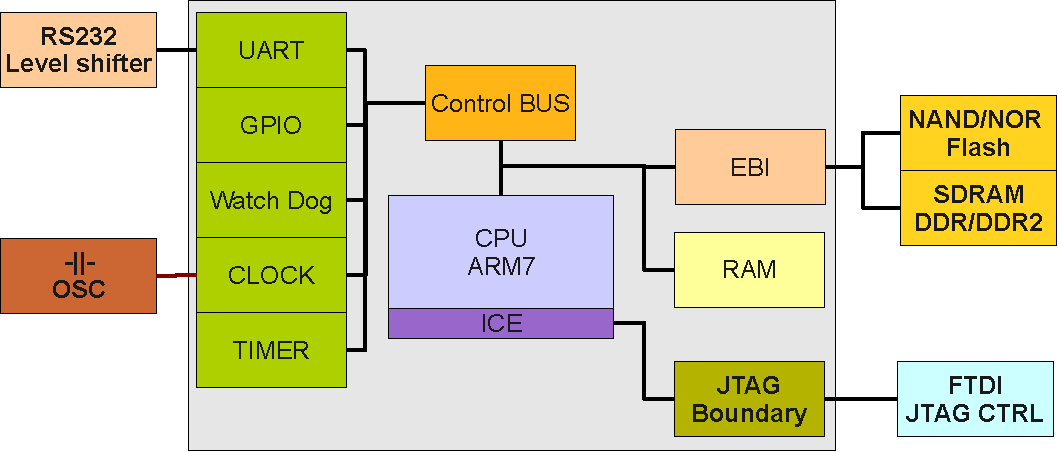
\includegraphics[scale=.25]{../images/ECB_ARM7_Block.pdf}}
            \subfigure{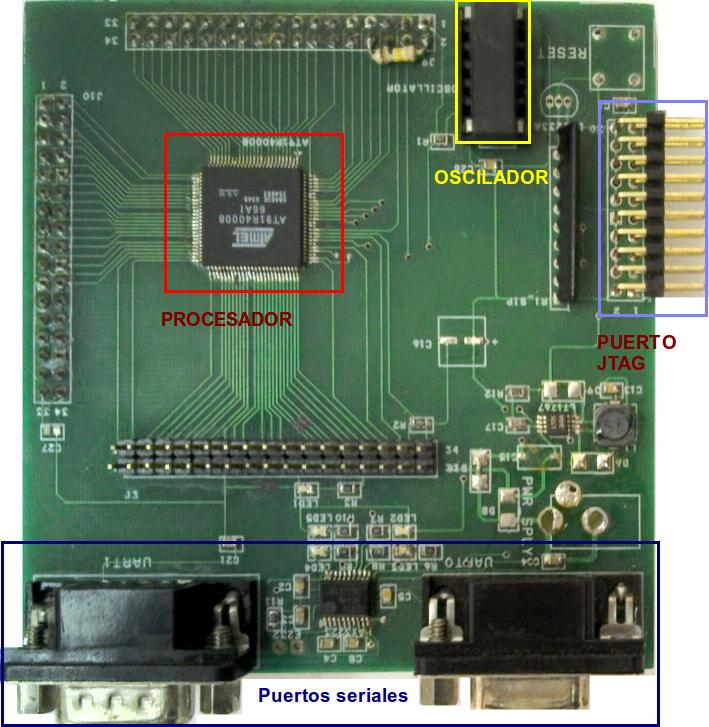
\includegraphics[scale=.2]{../images/ECB_ARM7.jpg}}
          }
    };

    \onslide<3> \node [ph_explain, right=.5cm of adaptation.east] (exp_adaptation)    
    {
      \begin{center} \textbf{Absorci�n: Plataforma Xport } \end{center}
      \centering
        \mbox{
          \subfigure{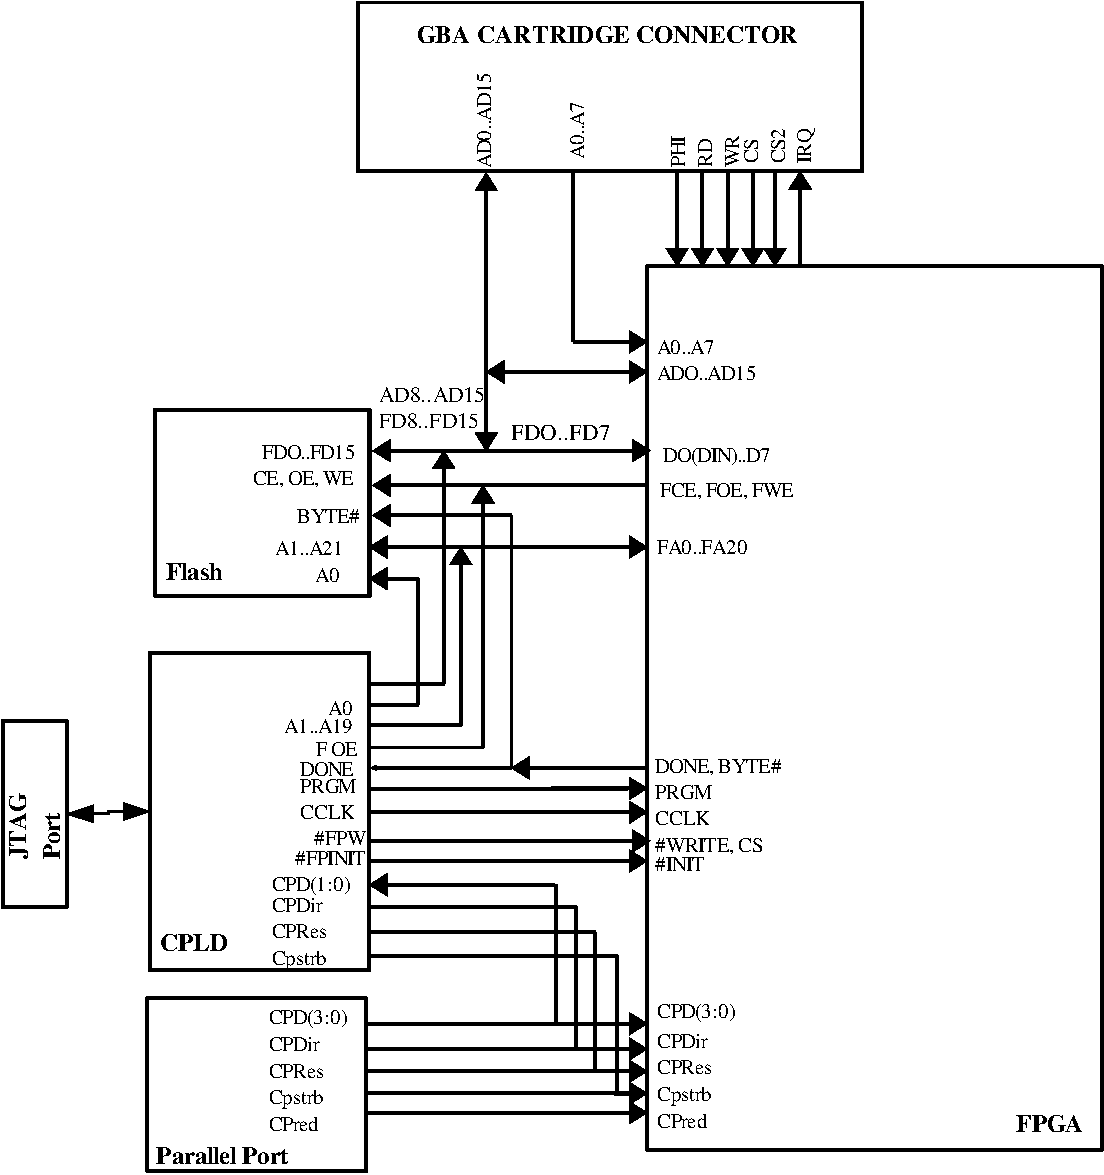
\includegraphics[scale=.28]{../images/xport_Block.pdf}}
          \subfigure{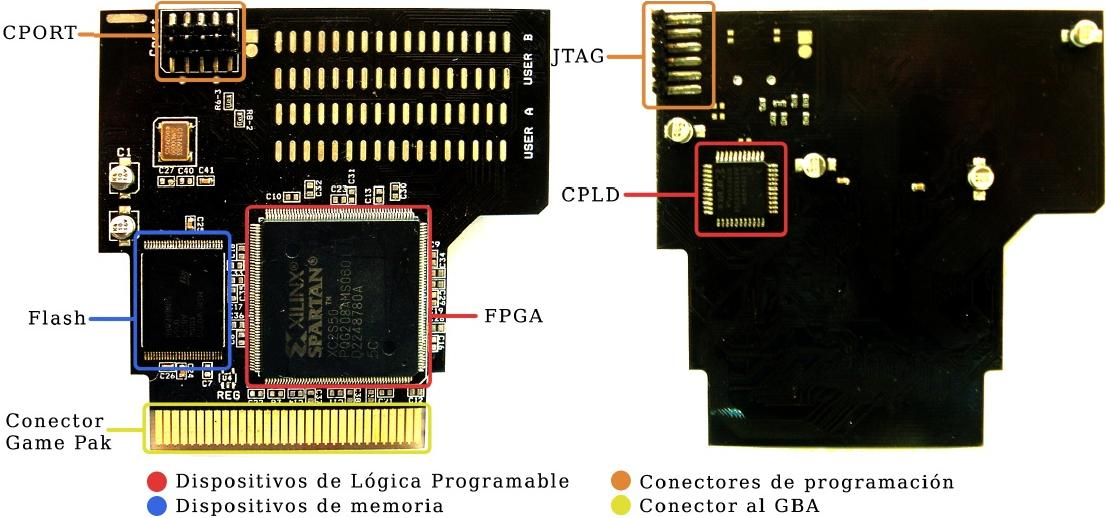
\includegraphics[scale=.2, angle=90]{../images/xport.jpg}}
        }
     };
 
    \onslide<4> \node [ph_explain, right=.5cm of adaptation.east] (exp_adaptation)    
    {
      \begin{center} \textbf{Absorci�n: Plataforma ECB\_AT91\_V1} \end{center}
      \centering
      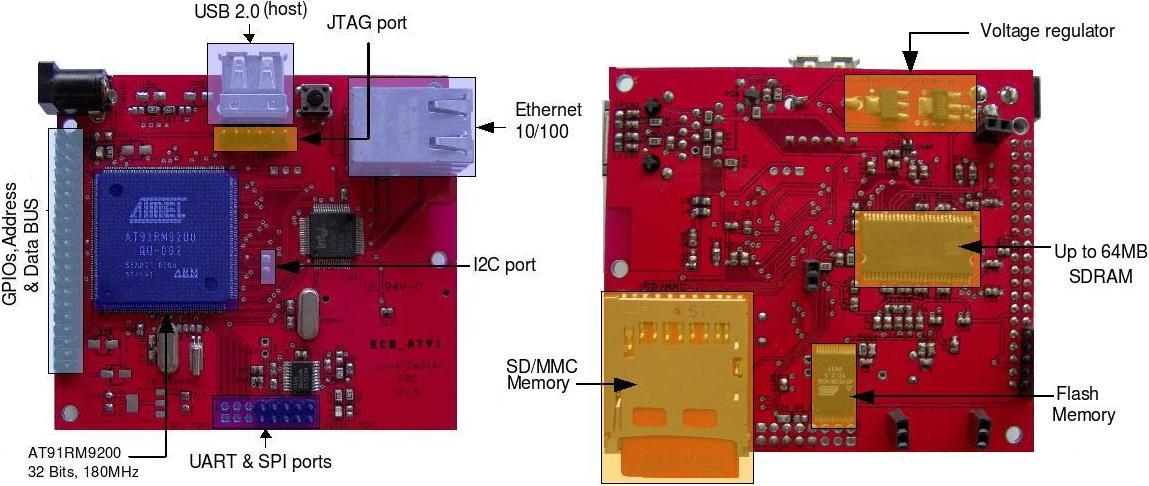
\includegraphics[scale=.3]{../images/ECB_AT91_V1.jpg}
    };

    \onslide<5> \node [ph_explain, right=.5cm of adaptation.east] (exp_adaptation)    
    {
      \begin{center} \textbf{Absorci�n: Plataforma ECB\_AT91\_V2} \end{center}
        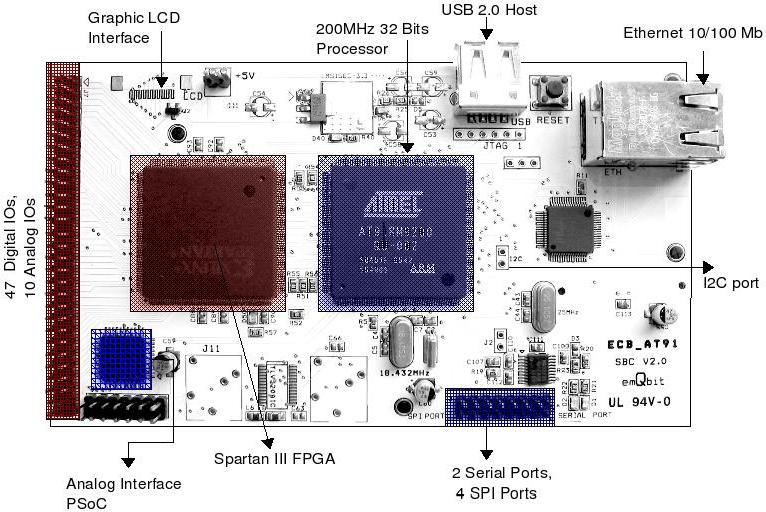
\includegraphics[scale=.43]{../images/ECB_AT91_V2.jpg}
    };
 
    \onslide<6> \node [ph_explain, right=.5cm of adaptation.east] (exp_adaptation)    
    {
      \begin{center} \textbf{Absorci�n: Plataforma ECBOT} \end{center}
      \centering
       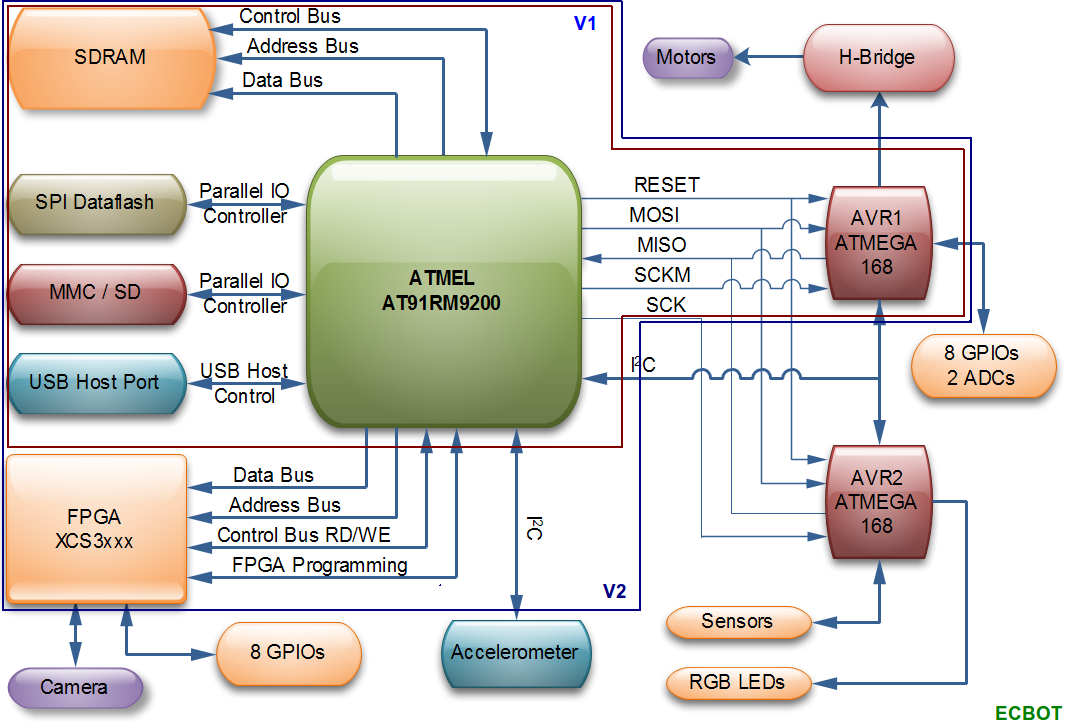
\includegraphics[scale=.2]{../images/ECBOT_Block.png} \\
       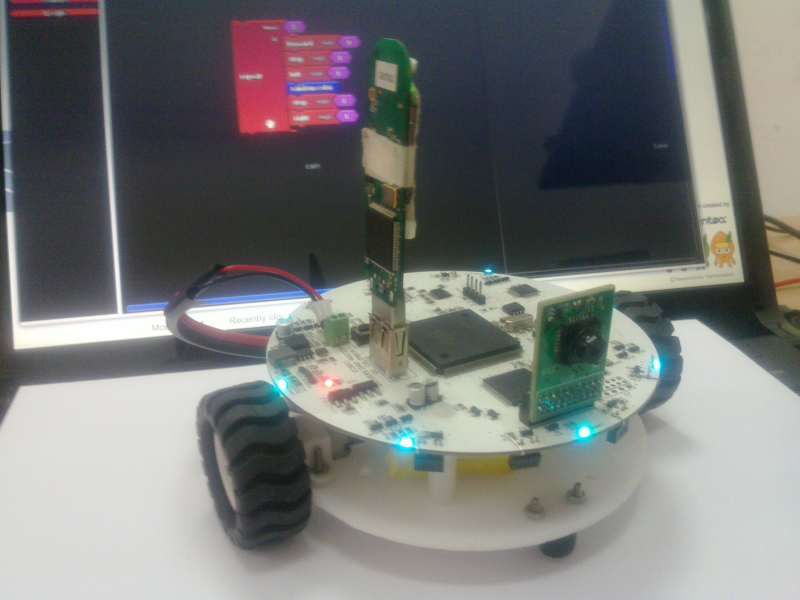
\includegraphics[scale=.2]{../images/ECBOT.png}
    };

    \onslide<7> \node [ph_explain, right=.5cm of adaptation.east] (exp_adaptation)    
    {
      \begin{center} \textbf{Absorci�n: Plataforma ECB\_BF532} \end{center}
     \centering
       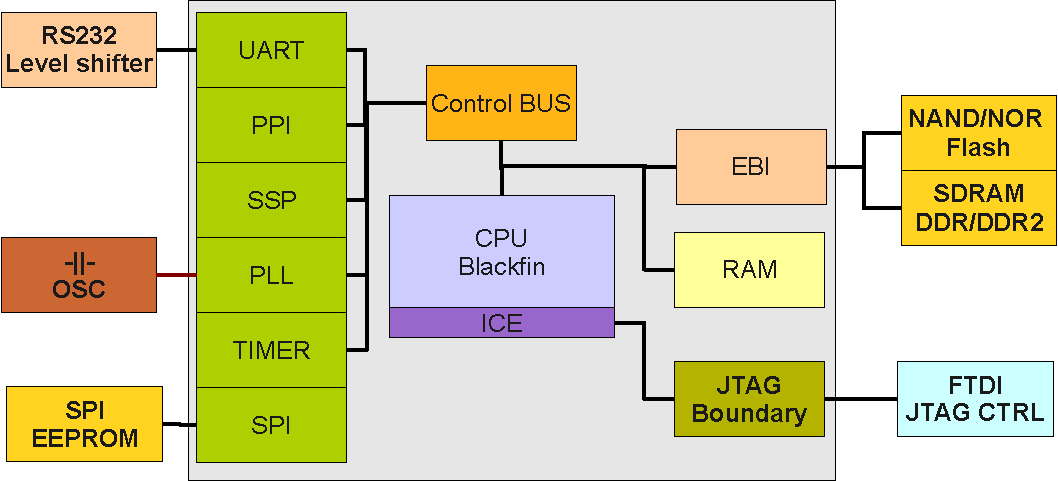
\includegraphics[scale=.25]{../images/ECB_BF532_Block.pdf} \\
       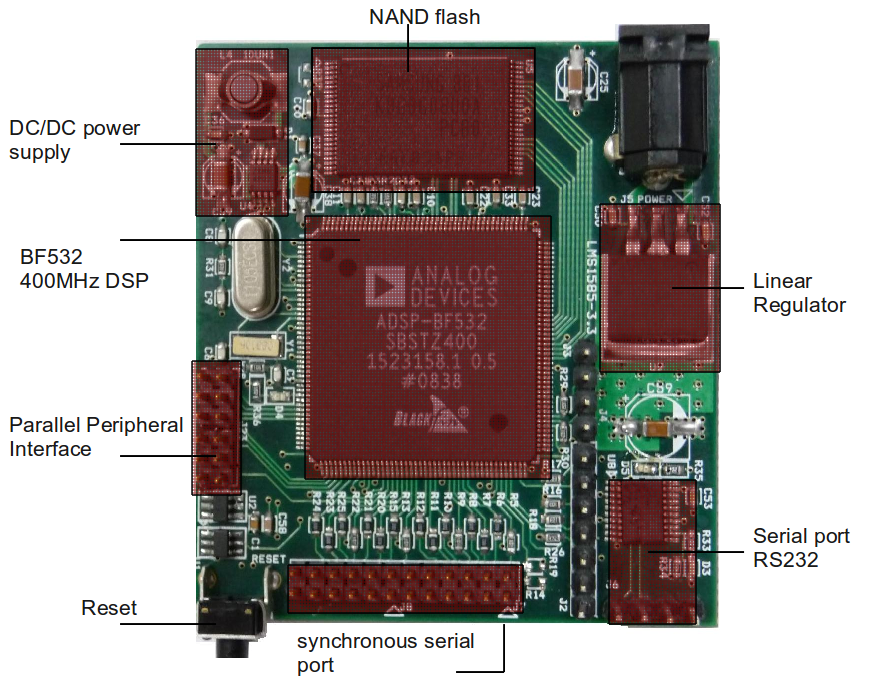
\includegraphics[scale=.25]{../images/ECB_BF532.png}
    };
 
    \onslide<8> \node [ph_explain, right=.5cm of adaptation.east] (exp_adaptation)    
    {
      \begin{center} \textbf{Absorci�n: Plataforma SIE } \end{center}
      \centering
      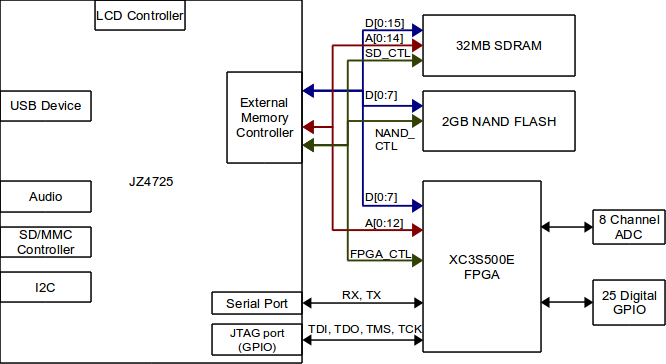
\includegraphics[scale=.3]{../images/SIE_block_diagram.png} \\
      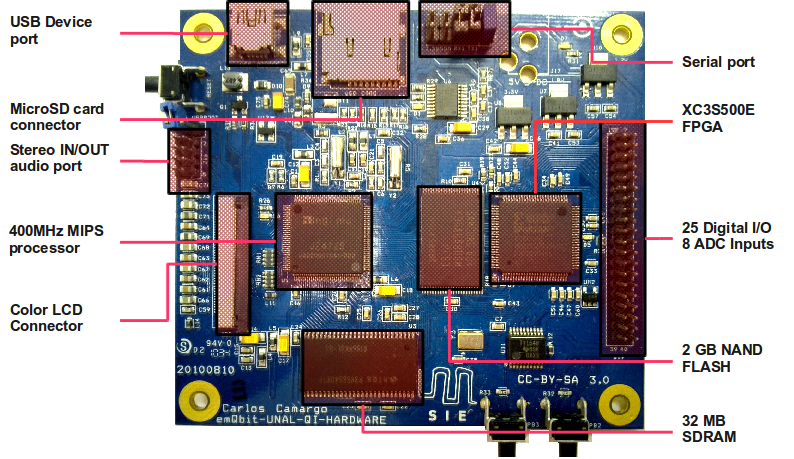
\includegraphics[scale=.3]{../images/SIE.jpg}
    };

    \onslide<9> \node [ph_explain, right=.5cm of adaptation.east] (exp_adaptation)    
    {
      \begin{center} \textbf{Absorci�n: Res�men plataformas } \end{center}
      \centering
        \resizebox{!}{.82cm}{
            \footnotesize
            \begin{tabular}{|l|l|l|l|l|l|l|}
              \hline
              \textbf{Plataforma} & \textbf{CPU}  & \textbf{Capas} 
                                                      & \textbf{Montaje}    & \textbf{Cant.}
                                                                                  &\textbf{OS} &\textbf{Usuario}
              \\ \hline 
              ECB\_ARM7          &ARM7,33M      & 2 & local Manual.       & 2   & eCos    & UN
              \\ \hline 
              UN\_UIS\_XPORT     &ARM7,50M      & 2 & local Manual.       & 2   & eCos    & UN, UIS
              \\ \hline 
              ECB\_AT91\_V1      &ARM920,180M   & 2 & local Manual/Autom. & 100 & Linux   & UN, UIS, ULA, ENAP, UDFJC, USTA
              \\ \hline 
              ECB\_AT91\_V2      &ARM920 180M   & 4 & local Manual.       & 30  & Linux   & UN, UIS, ULA, ENAP, UDFJC 
              \\ \hline 
              ECBOT              &ARM920 180M   & 4 & local Manual.       & 20  & Linux   & UN, UIS
              \\ \hline 
              ECB\_BF532         &Blackfin 400M & 4 & local Manual.       & 5   & uCLinux & UN
              \\ \hline 
              SIE                &MIPS32  300M  & 2 & externo Autom.      & 80  & Linux   & UN, UIS, ULA, ECI
              \\ \hline 
            \end{tabular}
     }
    };
   


    \onslide<10> \node [ph_explain, right=.5cm of adaptation.east] (exp_adaptation)    
    {
      \begin{center} \textbf{Absorci�n: Proceso de Fabricaci�n de PCBs} \end{center}
      \centering
      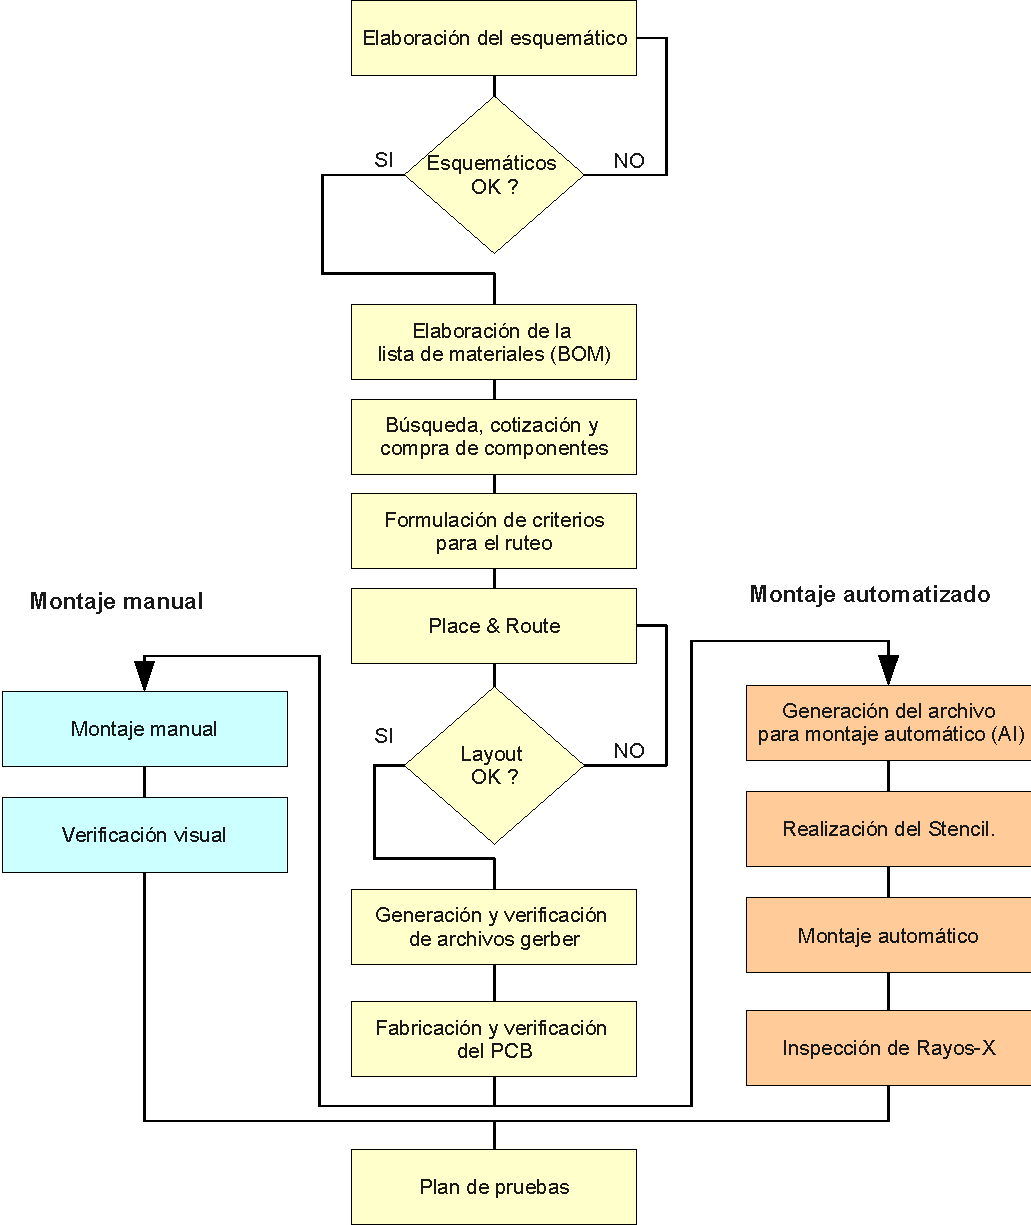
\includegraphics[scale=.35]{../images/proceso_de_fabricacion_PCBs.pdf}
    };

    \onslide<11> \node [ph_explain, right=.5cm of adaptation.east] (exp_adaptation)    
    {
      \begin{center} \textbf{Absorci�n: Flujo de ingenier�a inversa} \end{center}
      \centering
      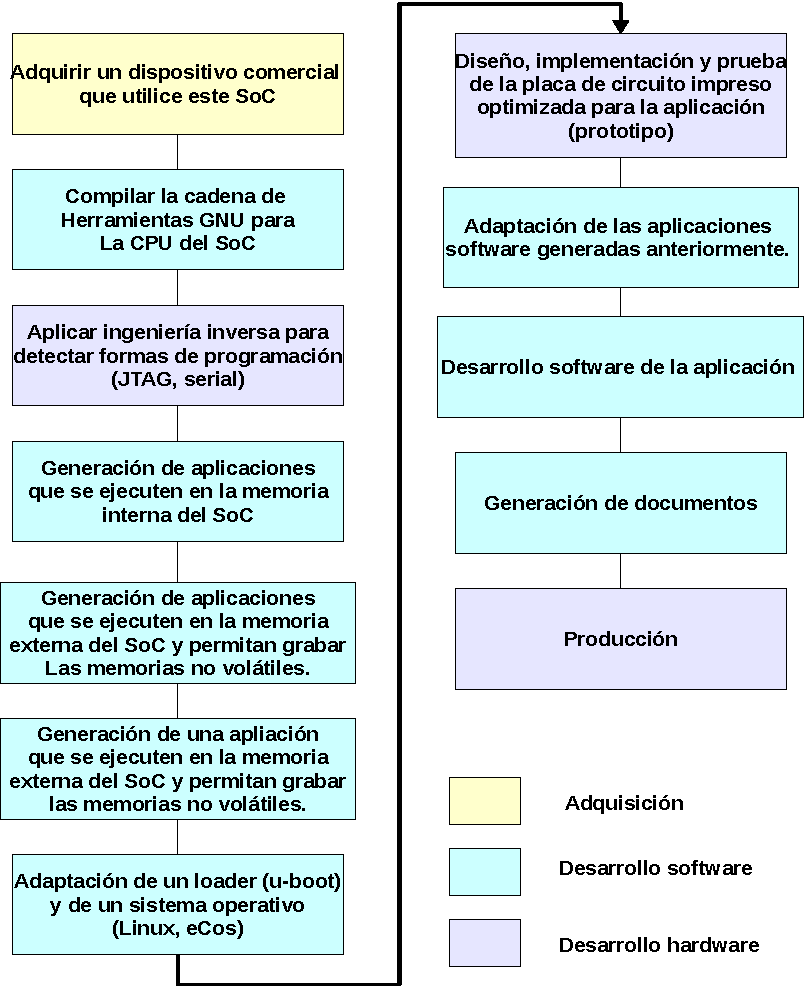
\includegraphics[scale=.37]{../images/SoC_reverse.pdf}
   };
 
\end{tikzpicture}
\end{figure}

\end{frame}